\documentclass[12pt]{article}
\usepackage{array}
\usepackage{amsmath}
\usepackage{amssymb}
\usepackage{algorithm}
\usepackage{algorithmic}
\usepackage{caption}
\usepackage{fontspec}
\usepackage{graphicx}
\usepackage{indentfirst}
\usepackage{minted}
\usepackage{mathtools}
\usepackage{pifont}
\usepackage{setspace}
\usepackage{subfigure}
\usepackage{tikz}
\usepackage{url}
\usepackage{xcolor}
\usepackage{xeCJK}

\usepackage[colorlinks=true]{hyperref}
\usepackage[margin=0.55in]{geometry}

% background color for minted
\definecolor{bg}{rgb}{0.95,0.95,0.95}

% CJK font
\setCJKmainfont{Source Han Serif CN}

% indent value
\setlength{\parindent}{2em}

% line spacing
\linespread{1.2}

\title{Introduction of The Perspective Projection Matrix}
\author{Yiteng Zhang}
%\date{}

\begin{document}
\maketitle

\indent{}透视投影可以说是图形学基础中的基础。为了从三维场景渲一幅二维图像出来,往往通过透视投影进行三维到二维
的转换过程。从计算的过程来看,虽然其实不过是几次矩阵操作,但正确理解其中的原理还是很重要的。想要找到靠谱而富含
细节的资料其实并不容易,然而幸运的是,目前Scratchapixel这个网站上有一些很好的讲解,这里对其中的相关内
容进行一些简要的总结。

\begin{figure}[h]
\centering
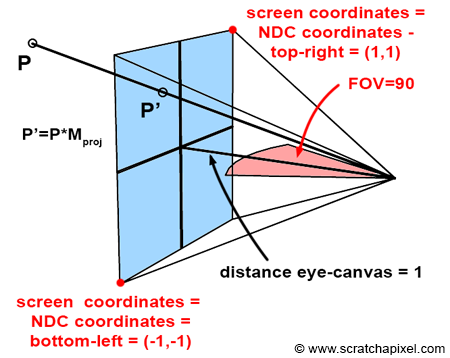
\includegraphics[width=7cm]{./imgs/perspprojmatrix2.png}
\end{figure}

\indent{}我们知道,可以通过透视投影将三维空间中的点$P$投影至画布(Canvas)所在的平面上,则可得到对应的点$P'$。如果我们再对%
$P'$的坐标做归一化,就可以得到它在NDC坐标系下的表达,对应的二维空间中的坐标可以表示为$(x',y')$。NDC坐标系具体的
取值范围并非在所有讨论中都是一样的,在实践中它的范围往往是$[-1,1]\in \mathbb{R}$,在当前讨论中我们也使用该范围,而非
在之前一些讨论中使用的$[0,1]\in \mathbb{R}$。实际上,这里往往只有API不同造成的差别,其内在的道理是一样的。

\begin{figure}[h]
\centering
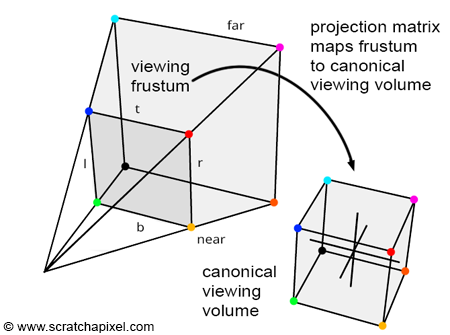
\includegraphics[width=7cm]{./imgs/canonical1.png}
\end{figure}

\indent{}实际上,$P'$在$x$,$y$和$z$三个方向的坐标值都会被重映射到$[-1,1]\in\mathbb{R}$ 或 $[0,1]\in\mathbb{R}$范围
上(这取决于我们用的API的相应规定),这意味着视锥体的那部分空间被映射到一个立方体的空间中。当然了,如果我们使用的
API将$z$轴坐标映射到$[0,1]\in\mathbb{R}$,那么确实不是一个立方体,因为映射后对应的是一个维度为$2\times 2\times 1$的
空间,$z$轴坐标被映射至$[-1,1]\in\mathbb{R}$时,才对应于一个维度为$2\times 2\times 2$的立方体空间。不过这个差别并不重要,
无论使用什么API,我们都是要将viewing frustum的空间映射到一个方的空间上,这个方的空间被称为 \textbf{Canonical Viewing Volume}。
这个映射过程实际上就是viewing frustum被归一化的过程,也就是projection matrix要做的事情。

\indent{}在之前的讨论中,我们将平移,旋转等变换描述为一个$4\times 4$矩阵。然而,笛卡尔坐标系中的一个三维点是$1\times 3$的,
我们没办法将三维点的坐标构成的向量与$4\times 4$的变换矩阵相乘。另一方面,如果我们打算使用$3\times 3$的矩阵来描述变换操作,
我们会发现它无法表达平移操作,只能通过再加上一个三维向量来表达平移,这种不统一的表达也不免让人不快。
在实践中,解决上述问题的方法是使用\textbf{齐次坐标系(Homogeneous Coordinate)}。
一个三维点在笛卡尔坐标系与齐次坐标系间的转换为:

\begin{displaymath}
\textrm{Cartesian Point }[x, y, z] \;\; \overset{\textrm{Implicit Conversion}}{\longrightarrow} \;\;
\textrm{Homogeneous Point }[x, y, z, w=1]
\end{displaymath}

\indent{}实际上,可以看到我们其实什么也不用做,我们在心里给笛卡尔坐标系的表达加上一维$w$,并让对应的坐标值为单位值即可,我们
可以随时将这个单位值丢掉,并以标准的三维笛卡尔坐标系的表达来表示三维点。这里我们使用了行主序来表示向量。

\indent{}需要注意的一点是,虽然在$w=1$时,我们可以随时丢掉最后一维以将齐次坐标转换为笛卡尔坐标。然而,在计算过程中$w$的值可
能并不为单位值,如果我们想要在这种情况下得到对应的笛卡尔坐标系下的表达,需要进行下述转换:
\begin{displaymath}
\textrm{Homogeneous Point }[x, y, z, w\neq 1] \;\; \overset{\textrm{Conversion}}{\longrightarrow} \;\;
[\frac{x}{w},\frac{y}{w},\frac{z}{w},\frac{w}{w}=1]
\;\; \rightarrow \;\; \textrm{Cartesian Point }[\frac{x}{w},\frac{y}{w},\frac{z}{w}]
\end{displaymath}

\indent{}我们将会看到,在齐次坐标系的表达下,平移操作可以很好地融入到一次矩阵乘法中。当我们将下面的以$4\times 4$矩阵
表达的变换应用到一个齐次坐标系下的三维点$[x,y,z,w=1]$上,其过程为:
\begin{displaymath}
\begin{bmatrix}
x' & y' & z' & w'
\end{bmatrix}
=
\begin{bmatrix}
x & y & z & w = 1
\end{bmatrix}
*
\begin{bmatrix}
\color{green}{m_{00}} & \color{green}{m_{01}} & \color{green}{m_{02}} & \color{blue}{0}\\
\color{green}{m_{10}} & \color{green}{m_{11}} & \color{green}{m_{12}} & \color{blue}{0}\\
\color{green}{m_{20}} & \color{green}{m_{21}} & \color{green}{m_{22}} & \color{blue}{0}\\
\color{red}{T_x} & \color{red}{T_y} & \color{red}{T_z} & \color{blue}{1}\\
\end{bmatrix}
\end{displaymath}
\noindent{}需要注意的是,因为我们现在使用的是行主序表达,所以变换由矩阵右乘来进行。

\indent{}如果我们仔细地观察上述矩阵乘法的计算过程,就可以看到齐次坐标系的妙处。齐次坐标系很好地将平移操作融入进
矩阵乘法中来表达为一次线性变换,上述过程实际上等价于:
\begin{displaymath}
\begin{bmatrix}
x' & y' & z'
\end{bmatrix}
=
\begin{bmatrix}
x & y & z
\end{bmatrix}
*
\begin{bmatrix}
\color{green}{m_{00}} & \color{green}{m_{01}} & \color{green}{m_{02}}\\
\color{green}{m_{10}} & \color{green}{m_{11}} & \color{green}{m_{12}}\\
\color{green}{m_{20}} & \color{green}{m_{21}} & \color{green}{m_{22}}\\
\end{bmatrix}
+
\begin{bmatrix}
\color{red}{T_x} & \color{red}{T_y} & \color{red}{T_z}
\end{bmatrix}
\end{displaymath}
\noindent{}上式表明,在齐次坐标系下,上述$4\times 4$矩阵对应的变换相当于是在笛卡尔坐标系下的一次仿射变换。

\indent{}实际上,我们关注的Projection Matrix要做的是投影变换,投影变换与仿射变换之间是有重要区别的。在仿射变换的过程中,
额外的那一维$w$的值始终是单位值,不会变化。然而,Projection Matrix的最右一列并不一定是$[0,0,0,1]^T$的形式,经过投影变换,
所得向量在$w$维度上的值并不一定是单位值,不能直接被丢弃。两种变换的不同之处影响了我们的变换操作的具体实现过程。

\indent{}对于两种变换,我们都要将一个$4\times 4$矩阵与一个三维向量相乘。在实现时,我们完全可以将三维向量隐式地看作四维(加上一维$w$
并让其值为单位值),这意味着我们将要实现的函数的输入和输出都是三维向量,而不是显式的四维向量,这样的形式可以节省空间。

\indent{}对于仿射变换,因为在变换作用之后$w$的值不变,始终为$1$,我们可以直接省去矩阵乘法中$w$维度上的计算过程,相应的变换
函数可以实现为:
\begin{minted}[mathescape=true,
               linenos,
               numbersep=5pt,
               autogobble,
               frame=lines,
               fontsize=\small,
               bgcolor=bg,
               framesep=2mm]{C++}
    template<typename T>
    void affineTransform(const Vec3<T>& src, Vec3<T>& dst) {
        // the value of dst vector
        // value on w is always 1, so we need not to define it
        T a, b, c;

        // m is affine transformation matrix
        a = src.x * m[0][0] + src.y * m[1][0] + src.z * m[2][0] + m[3][0];
        b = src.x * m[0][1] + src.y * m[1][1] + src.z * m[2][1] + m[3][1];
        c = src.x * m[0][2] + src.y * m[1][2] + src.z * m[2][2] + m[3][2];

        // division by w is not necessary, w is 1
        dst.x = a;
        dst.y = b;
        dst.z = c;
    }
\end{minted}

\indent{}与仿射变换不同,投影变换并不能保证所得向量在$w$维度上的值为单位值。如果我们想将一个$w$上的值不为$1$的齐次坐标系下的向量
转换为笛卡尔坐标系下的表达,我们需要正确地计算$w$的值。如果考虑到这一点,我们可以给出对应的实现:
\begin{minted}[mathescape=true,
               linenos,
               numbersep=5pt,
               autogobble,
               frame=lines,
               fontsize=\small,
               bgcolor=bg,
               framesep=2mm]{C++}
    template<typename T>
    void multVecMatrix(const Vec3<T>& src, Vec3<T>& dst) {
        // the value of dst vector
        T a, b, c, w;

        // m may be the projection matrix
        a = src.x * m[0][0] + src.y * m[1][0] + src.z * m[2][0] + m[3][0];
        b = src.x * m[0][1] + src.y * m[1][1] + src.z * m[2][1] + m[3][1];
        c = src.x * m[0][2] + src.y * m[1][2] + src.z * m[2][2] + m[3][2];
        w = src.x * m[0][3] + src.y * m[1][3] + src.z * m[2][3] + m[3][3];

        if (w != 1) {
            dst.x = a / w;
            dst.y = b / w;
            dst.z = c / w;
        } else {
            dst.x = a;
            dst.y = b;
            dst.z = c;
        }
    }
\end{minted}

\noindent{}上述的\texttt{multVecMatrix}实现可以正确地处理投影变换过程,对仿射变换也可以很好地工作。

\indent{}现在我们对变换矩阵有了一些了解,接下来就要进一步根据透视投影的过程推出与透视投影变换对应的矩阵,也可以
说是\textbf{透视投影矩阵(Perspective Projection Matrix)}。

\indent{}从透视投影的原理可以知道,三维点$P$在像平面上的投影点$P'$的位置可以通过z-divide得到,由于相机坐标系的$z$轴
方向是朝着相机屏幕向内的,我们要考虑到方向性,因而z-divide 的过程是:

\begin{displaymath}
P_{x}' = \frac{P_x}{-P_z}, \;\;\;\; P_{y}' = \frac{P_y}{-P_z}
\end{displaymath}

\indent{}我们的目标是将z-divide的过程用矩阵乘法来表达,问题在于相应的$4\times 4$矩阵应该是何种形式呢?回想起齐次坐标与
笛卡尔坐标的转换过程,如果$w$的值不为单位值,我们就要做division。从这一点出发,就可以发现,我们可以想办法让经过投影
变换后的$w$值为$-P_z$,然后通过齐次坐标到笛卡尔坐标的转换来完成z-divide过程,所以可以写出:

\begin{displaymath}
\begin{bmatrix}
x & y & -z & -z
\end{bmatrix}
=
\begin{bmatrix}
x & y & z & 1
\end{bmatrix}
*
\begin{bmatrix}
1 & 0 & 0 & 0\\
0 & 1 & 0 & 0\\
0 & 0 & -1 & \color{red}{-1}\\
0 & 0 & 0 & 0
\end{bmatrix}
\end{displaymath}

\noindent{}然后再将$[x,y,-z,-z]$转换到笛卡尔坐标系下的表示,得到$[x/-z,y/-z,1]$,这正是我们想要的。总结一下,
上述过程将点$P$投影至$P'$,其表达为:

\begin{displaymath}
\begin{bmatrix}
x' & y' & z'
\end{bmatrix}
=
\begin{bmatrix}
\dfrac{x}{-z} & \dfrac{y}{-z} & 1
\end{bmatrix}
\end{displaymath}

\indent{}现在我们有了一个简单的透视投影矩阵,但仍然有很多细节需要考虑。主要有两点,首先,根据一开始所说的,我们还需要
将$z'$重映射到$[0,1]\in\mathbb{R}$或$[-1,1]\in\mathbb{R}$。为了做到这一点,我们要用到相机的\textbf{近剪裁平面(near
clipping plane)}和\textbf{远剪裁平面(far clipping plane)}。另外,我们还要考虑相机的\textbf{视场(field-of-view)},
它控制着我们(的相机)可以看到多少场景。

\indent{}Perspective Projection Matrix 会将$z$坐标值归一化,这里我们不妨将归一化的目标范围设定为$[0,1]\in\mathbb{R}$。
在这种情况下,经过z-divide后,近剪裁平面上的的点会被映射到$z'=0$,远剪裁平面上的点会被映射到$z'=1$。如果近剪裁平面
距相机坐标系原点距离为$n$,远剪裁平面距相机坐标系原点距离为$f$,那么我们可以得到新的透视投影矩阵:

\begin{displaymath}
\begin{bmatrix}
1 & 0 & 0 & 0 \\
0 & 1 & 0 & 0 \\
0 & 0 & \color{red}{-\dfrac{f}{(f-n)}} & -1\\
0 & 0 & \color{red}{-\dfrac{f*n}{(f-n)}} & 0\\
\end{bmatrix}
\end{displaymath}

\noindent{}简单验证一下,对于近剪裁平面和远剪裁平面上的点,分别有$z=-n$和$z=-f$,那么:
\begin{align*}
&\textrm{for points on near clipping plane: }z' = \dfrac{\dfrac{(-n)*(-f)}{(f-n)} - \dfrac{f*n}{(f-n)}}{-(-n)} = 0\\
&\textrm{for points on far clipping plane: }z' = \dfrac{\dfrac{(-f)*(-f)}{(f-n)} - \dfrac{f*n}{(f-n)}}{-(-f)} = 1
\end{align*}
\noindent{}我们目前先给出该矩阵的形式,在后面会具体地阐述这两个参数的推导过程。

\begin{figure}[h]
\centering
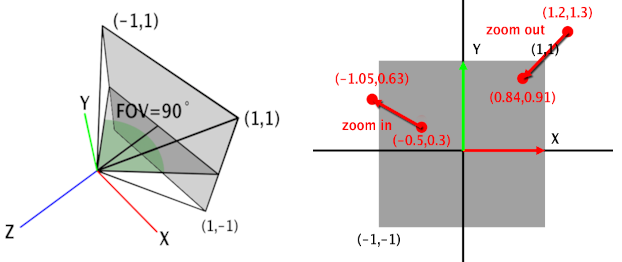
\includegraphics[width=9cm]{./imgs/camsetup1.png}
\end{figure}

\indent{}Perspective Projection Matrix会将$x$与$y$的值映射至$[-1,1]\in\mathbb{R}$范围内,以得到点在NDC坐标系下的坐标值。
我们可以说,屏幕窗口(screen window)的尺寸是$-1\sim 1$,在这个范围内的点是可见的。需要说明的是,无论FOV是多少,屏幕窗口的
尺寸是不会变的。这似乎有些反直觉,在一般观念上,如果FOV改变了,窗口尺寸应该也会随之改变,但这不是矛盾了吗?实际上,如果
我们希望屏幕尺寸固定的话,真正改变的其实是投影点的坐标,我们对其坐标值进行缩放并检查它是否仍落在屏幕内部。具体来说,如果
我们减少\textbf{焦距(focal length)},即增大FOV,相当于镜头发生zoom out,原本不可见的一些点会成为可见的。如果反过来,
减小FOV,则相当于镜头发生zoom in,一些原本可见的点会变得不可见。无论是哪种情况,我们的screen window尺寸并不改变。

\indent{}出于计算方便的考虑,实践中的FOV往往是上述讨论中的角度的一半。在这里,为了表述上的便利,我们定义FOV为整个
角度。实际用到的FOV可以是水平角或垂直角,上图中我们给出的是对应于水平角的FOV。如果screen window是
方的,即其\textbf{宽高比(aspect ratio)}是$1$,那么具体采用哪个方向并无差别,因为角度是一样的。但如果不是这种
情况,就需要明确我们使用的是定义在哪个方向上的FOV了。在实践中,OpenGL采用的是垂直角,我们在这里采用了水平角。

\indent{}为了将上述zoom out 与 zoom in 动作融入到目前的$4\times 4$透视投影矩阵中,我们需要对$x$与$y$的坐标值做scaling。
假设screen是方的,并假设screen到眼的距离是单位距离,则根据简单的三角关系可以给出缩放因子$S$的表达,并得到更加完善
的透视投影矩阵:
\begin{displaymath}
S = \frac{1}{\tan\bigg(\dfrac{fov}{2} * \dfrac{\pi}{180}\bigg)}
\quad\quad
M=
\begin{bmatrix}
\color{red}{S} & 0 & 0 & 0 \\
0 & \color{red}{S} & 0 & 0 \\
0 & 0 & -\dfrac{f}{(f-n)} & -1\\
0 & 0 & -\dfrac{f*n}{(f-n)}& 0\\
\end{bmatrix}
\end{displaymath}

\indent{}上面我们给出了透视投影矩阵的一种形式,但很显然透视投影矩阵的形式取决于很多约定。在OpenGL中使用的
透视投影矩阵就和上面的形式有一些差别。OpenGL假设场景中的点被投影至近剪裁平面上,而不是距相机位置单位距离的平面。
我们需要仔细地检查一些约定,我们要明确矩阵和向量的形式是行主序还是列主序,我们要明确坐标系是左手系还是右手系,
这些细节会影响透视投影的具体实现方式。不过,抛开这些细节来看的话,内在的原理是完全相同的。

\indent{}现在让我们来看看OpenGL中使用的Perspective Projection Matrix的具体形式,它与我们上述讨论中给出的矩阵形式
有些许不同。可以用\texttt{glFrustum}函数创建如下定义的透视投影矩阵:
\begin{displaymath}
\left[\begin{array}{cccc}
{ \dfrac{2n}{ r-l } } & 0 & { \dfrac{r + l} { r-l } } & 0 \\
0 & { \dfrac{2n}{ t-b } } & { \dfrac{t + b}{ t-b } } & 0 \\
0 & 0 & -{\dfrac{f+n}{f-n}} & -{\dfrac{2fn}{f-n}}\\
0 & 0 & -1& 0\\
\end{array}\right]
\end{displaymath}

\indent{}首先需要注意的是,OpenGL使用列主序约定,而我们之前的讨论一直在用行主序约定。通过简单的矩阵转置,我们可以
将上面这个列主序表达的矩阵转换为行主序的表达:
\begin{displaymath}
\left[\begin{array}{cccc}
{ \dfrac{2n}{ r-l } } & 0 & 0 & 0 \\
0 & { \dfrac{2n}{ t-b } } & 0 & 0 \\
{ \dfrac{r + l}{ r-l } } & { \dfrac{t + b}{ t-b } } & -{\dfrac{f+n}{f-n}} & {-1}\\
0 & 0 & -{\dfrac{2fn}{f-n}}& 0\\
\end{array}\right]
\end{displaymath}
\noindent{}可以发现这个矩阵的形式和我们之前给出的形式是非常相似的。

\begin{figure}[h]
\centering
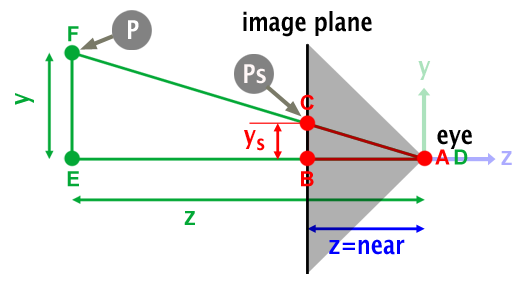
\includegraphics[width=8cm]{./imgs/projectionOpenGL.png}
\end{figure}

\indent{}我们很清楚透视投影的主要过程,就是做z-divide操作。不过,在之前的一些讨论中,我们一直假设投影平面
到相机中心的距离是单位距离,但这并不总是成立的。在OpenGL中,投影平面(即像平面)的位置被设定为近剪裁平面。
现在,我们设(位于近剪裁平面的)像平面到相机中心(即眼的位置)的距离是$n$,根据$\triangle ABC$与$\triangle DEF$的
三角形相似关系可知:

\begin{displaymath}
\frac{AB}{DE} = \frac{BC}{EF} \;\Rightarrow\; \frac{n}{-P_z} = \frac{BC}{P_y}
\end{displaymath}

\noindent{}BC 即为投影点Ps在相机坐标系的$y$轴方向上的坐标:
\begin{displaymath}
BC = Ps_{y} = \frac{n*P_y}{-P_z}
\end{displaymath}
可以发现,这个形式和前述简单z-divide形式的差别仅仅是多出一个因子,这个因子正是像平面到相机中心的距离。
相似的,投影点在$x$轴方向上的坐标为:
\begin{displaymath}
Ps_x = \frac{n*P_x}{-P_z}
\end{displaymath}

\indent{}回忆一开始提到的,透视投影矩阵的作用是将viewing frustum重映射,将其warp到一个unit cube空间。我们在这里
再次给出之前的示意图:

\begin{figure}[h]
\centering
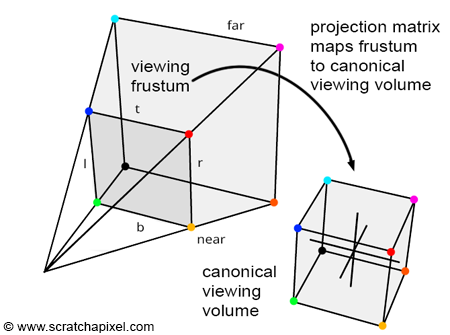
\includegraphics[width=8cm]{./imgs/canonical1.png}
\end{figure}

\indent{}该图即为OpenGL的透视投影矩阵的作用。与我们已经得到的透视投影矩阵的形式不同,在定义OpenGL的透视投影矩阵
时,相机的screen的具体尺寸由四个参数$l$,$r$,$t$和$b$给出。这四个值构成了screen左下角与右上角的坐标值,分别为$(l,b)$
与$(r,t)$。经过透视投影变换后,所得到的Canonical volume确实是一个立方体,因为其$x$,$y$
与$z$的坐标值的范围均在$[-1,1]\in\mathbb{R}$上。如果投影点$Ps$是可见的,那么其$x$坐标值需要满足:

\begin{displaymath}
l \leqslant Ps_x \leqslant r
\end{displaymath}

\noindent{}因为$Ps_x$的值会被重映射至$[-1,1]\in\mathbb{R}$,那么不等式两侧的值的形式应被重写:
\begin{displaymath}
l \leqslant Ps_x \leqslant r \;\Rightarrow\; -1 \leqslant 2\frac{Ps_x-l}{r-l}-1 \leqslant 1
\end{displaymath}
\noindent{}然后我们再将$Ps_x$写成z-divide的形式,则有:

\begin{displaymath}
-1 \leqslant 2\frac{Ps_x-l}{r-l}-\frac{r-l}{r-l} \leqslant 1 \;\Rightarrow\;
-1 \leqslant \frac{2nP_x}{-P_z (r-l)} - \frac{r+l}{r-l} \leqslant 1
\end{displaymath}

\noindent{}有关$Ps_y$的推导过程也是相同的,可以得到:

\begin{displaymath}
-1 \leqslant \frac{2nP_y}{-P_z(t-b)} - \frac{t+b}{t-b} \leqslant 1
\end{displaymath}

\noindent{}至此我们已经推出了OpenGL透视投影矩阵中有关$x$与$y$坐标的参数。

\indent{}透视投影矩阵中有关$z$坐标的相关参数的推导要稍稍复杂一点。在OpenGL中,$z$的坐标值会被映射至$[-1,1]\in\mathbb{R}$内。
对于近剪裁平面上的点,其$z$坐标被映射至$-1$。对于远剪裁平面上的点,其$z$坐标被映射至$1$。通过矩阵乘法,我们知道
$Ps_z$的表达应该是:

\begin{displaymath}
Ps_z = \frac{0*P_x + 0 * P_y + A * P_z + B * 1}{-P_z} = \frac{AP_z + B}{-P_z}
\end{displaymath}

\noindent{}其中A与B是有关$z$坐标重映射的两个相关参数。

\indent{}针对上式,我们分别将近剪裁平面上的点(对应的$P_z=-n$)和远剪裁平面上的点(对应的$P_z=-f$)对应的值
代入,则可得到两个方程构成的方程组:

\begin{displaymath}
\left\{ \begin{array}{ll} {-nA + B} = -n\\
{-fA + B} = f \end{array} \right.
\end{displaymath}

\noindent{}解这个简单的方程组即可得到两个参数的值:

\begin{displaymath}
A = -\frac{f+n}{f-n}, \quad\; B = -\frac{2fn}{f-n}
\end{displaymath}

\noindent{}至此,我们已经推导出OpenGL所用的透视投影矩阵的所有相关参数。

\indent{}根据上述推导,我们得到了OpenGL的Perspective Projection Matrix的最终形式,它由六个参数定义,
即$l$,$r$,$t$,$b$,$n$和$f$。其中,近剪裁平面的位置$n$与远剪裁平面的位置$f$由用户直接定义。但是,
剩下的四个与screen相关的参数是从何而来呢?实际上,它们是通过相机的field of view 与screen的aspect ratio
计算而来的,只需要用到简单的三角关系。

\begin{figure}[h]
\centering
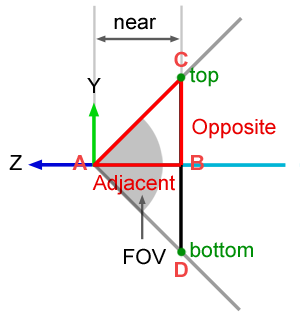
\includegraphics[width=5.2cm]{./imgs/openglsetup.png}
\end{figure}

\noindent{}给定aspect ratio的值$\phi$,field of view 的值 $fov$,则所求的四个参数的值为:
\begin{align*}
&t = \tan(fov/2) * n\\
&b = -t\\
&r = t * \phi\\
&l = -r
\end{align*}
\indent{}在实践时,我们实际需要四个参数$\phi$,$fov$,$n$与$f$。首先通过前三个参数计算出$l$,$r$,$t$与$b$,
再用所有需要的六个参数构建出透视投影矩阵。

\end{document}